\documentclass[12pt]{standalone}

\usepackage{tikz}

\begin{document}
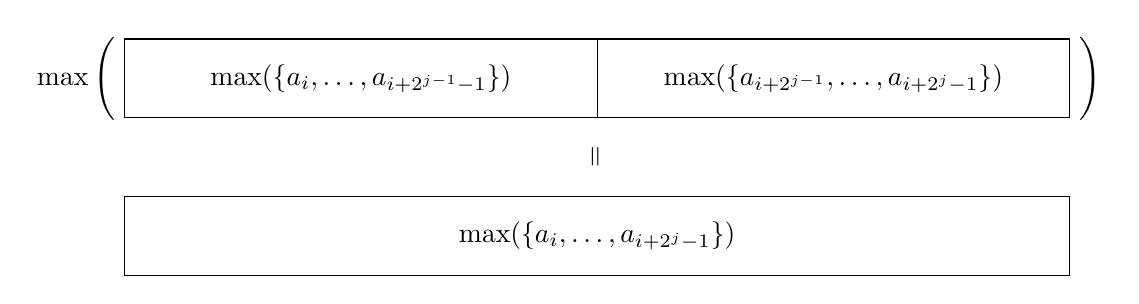
\begin{tikzpicture}[x=1cm,y=1cm]

\node[left] at (0,2.5) {$\max\Bigg($};
\node[right] at (12,2.5) {$\Bigg)$};

\draw (0,3) rectangle
    node {$\max(\{a_i, \dots, a_{i+2^{j-1}-1}\})$}
    ++(6,-1);
\draw (6,3) rectangle
    node {$\max(\{a_{i+2^{j-1}}, \dots, a_{i+2^j-1}\})$}
    ++(6,-1);

\node at (6,1.5) {\rotatebox{90}{$=$}};

\draw (0,1) rectangle node {$\max(\{a_i, \dots, a_{i+2^j-1}\})$}
    ++(12,-1);

\end{tikzpicture}
\end{document}
